\documentclass[12pt]{article}

% a template that a friend gave, it's worked well enough for me
% i have added some packages and stuff that have proved useful

\usepackage{fancyhdr}
\usepackage{tipa}
\usepackage{fontspec}
\usepackage{amsfonts}
\usepackage{enumitem}
\usepackage[margin=1in]{geometry}
\usepackage{graphicx}
\usepackage{float}
\usepackage{amsmath}
\usepackage{braket}
\usepackage{amssymb}
\usepackage{booktabs}
\usepackage{hyperref}
\usepackage{mathtools}
\usepackage{xcolor}
\usepackage{float}
\usepackage{algpseudocodex}
\usepackage{titlesec}
\usepackage{bbm}

\pagestyle{fancy}
\fancyhf{} % sets both header and footer to nothing
\lhead{Kevin Sheng}
\setmainfont{Comic Neue}
\renewcommand{\headrulewidth}{1pt}
\setlength{\headheight}{0.75in}
\setlength{\oddsidemargin}{0in}
\setlength{\evensidemargin}{0in}
\setlength{\voffset}{-.5in}
\setlength{\headsep}{10pt}
\setlength{\textwidth}{6.5in}
\setlength{\headwidth}{6.5in}
\setlength{\textheight}{8in}
\renewcommand{\headrulewidth}{0.5pt}
\renewcommand{\footrulewidth}{0.3pt}
\setlength{\textwidth}{6.5in}
\usepackage{setspace}
\usepackage{multicol}
\usepackage{float}
\setlength{\columnsep}{1cm}
\setlength\parindent{24pt}
\usepackage [english]{babel}
\usepackage [autostyle, english = american]{csquotes}
\MakeOuterQuote{"}

\setlength{\parskip}{6pt}
\setlength{\parindent}{0pt}

\titlespacing\section{0pt}{12pt plus 4pt minus 2pt}{0pt plus 2pt minus 2pt}
\titlespacing\subsection{0pt}{12pt plus 4pt minus 2pt}{0pt plus 2pt minus 2pt}
\titlespacing\subsubsection{0pt}{12pt plus 4pt minus 2pt}{0pt plus 2pt minus 2pt}

\hypersetup{colorlinks=true, urlcolor=blue}

\newcommand{\correction}[1]{\textcolor{red}{#1}}


\begin{document}
\begin{enumerate}
    \item The characteristic equation of this differential equation is $\lambda^2 - 4\lambda+13=0$.
          The solutions to this quadratic are
          \[\lambda=\frac{4 \pm \sqrt{16-52}}{2}=2 \pm 3i\]

          Since these are complex roots, we get that all solutions must take the form
          \begin{gather*}
              y=C_1e^{2t}\cos(3t)+C_2e^{2t}\sin(3t) \\
              y'=C_1e^{2t}(2\cos(3t)-3\sin(3t))+C_2e^{2t}(2\sin(3t)+\cos(3t))
          \end{gather*}

          Now, solving for initial conditions, we know that
          \begin{gather*}
              y(0)=C_1=4 \\
              y'(0)=2C_1+3C_2=0
          \end{gather*}
          From this, we get that $C_1=4$ and $C_2=-\frac{8}{3}$, which gives us our final solution
          \[\boxed{y=4e^{2t}\cos(3t)-\frac{8}{3}e^{2t}\sin(3t)}\]
    \item Let's set $x=0$ as when our spring is \textit{unstretched}.
          This gives us the following differential equation and initial conditions:
          \begin{align*}
              mx''=-kx-mg &  & x(0)=-\frac{0.1g}{3.6} &  & x'(0)=-0.4
          \end{align*}
          For readability reasons, I have replaced the mass and spring constant with $m$ and $k$ respectively.
          $g$ is the acceleration due to Earth's gravity (approx. $9.81 \frac{m}{s^2}$).

          Moving the terms around, we have
          \[\frac{m}{k}x''+x+\frac{mg}{k}=0\]
          To turn this equation homogeneous, we make the substitution $u=x+\frac{mg}{k}$:
          \[\frac{m}{k}u''+u=0 \rightarrow u''+\frac{k}{m}u=0\]
          We know this equation has the solution
          \begin{align*}
              u=A\cos\left(\omega t+\phi\right) &  & \omega=\sqrt{\frac{k}{m}}
          \end{align*}
          and substituting $x$ back in, we have
          \begin{gather*}
              x=A\cos\left(\omega t+\phi\right)-\frac{mg}{k} \\
              x'=-A\omega\sin(\omega t+\phi)
          \end{gather*}

          It remains to solve for initial conditions:
          \begin{gather*}
              -\frac{0.1g}{3.6}=A\cos \phi - \frac{0.1g}{3.6} \\
              -0.4=-A\sqrt{\frac{3.6}{0.1}}\sin \phi
          \end{gather*}

          Solving this system of equations gives us
          \begin{align*}
              A =\frac{1}{15} &  & \phi = \frac{\pi}{2} &  & \omega = 6
          \end{align*}
          \begin{center}
              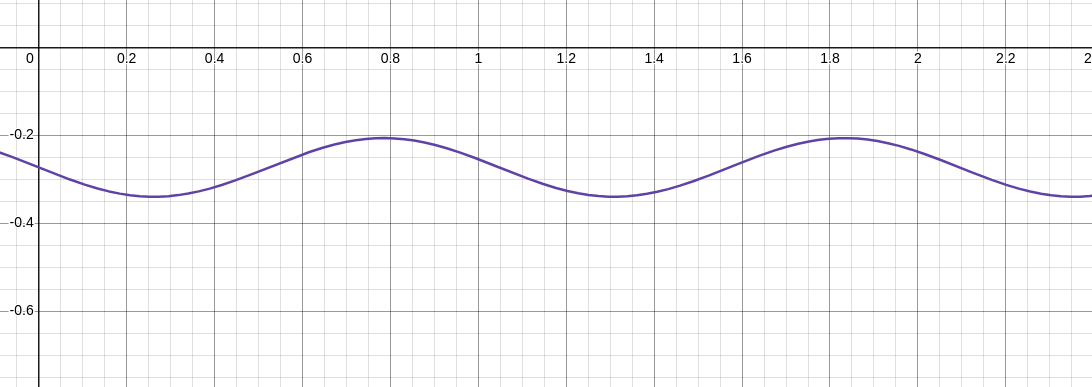
\includegraphics[height=5cm]{img/sho} \\
              \textit{A graph of the described motion.}
          \end{center}
    \item I believe there might be a typo in the original question.
          For clarity, this is the set of equations I am solving.
          \begin{align*}
              mx''+kx=0 &  & x(0)=x_0 &  & x'(0)=v_0
          \end{align*}
          We know that the solution to the first equation takes the form of
          \begin{gather*}
              x=a\cos(\omega t)+b\sin(\omega t) \\
              x'=-a\omega\sin(\omega t)+b\omega\cos(\omega t)
          \end{gather*}
          where $a$ and $b$ are constants.

          Solving for initial conditions, we have
          \begin{gather*}
              x_0=a \\
              v_0=b\omega \rightarrow b=\frac{v_0}{\omega}
          \end{gather*}
          Since $a=A\cos(\phi)$ and $b=A\sin(\phi)$, we have
          \begin{align*}
              a^2+b^2 & =A^2\left(\cos^2(\phi)+\sin^2(\phi)\right) \\
                      & =A^2                                       \\
                      & =x_0^2+\frac{v_0^2}{\omega^2}
          \end{align*}
          Then, solving the final equality, we get
          \[A=\sqrt{x_0^2+\frac{v_0^2}{\omega^2}}=\sqrt{x_0^2+\frac{m}{k}v_0^2}\quad\square\]
    \item The forcing term is $e^{-2t}$.
          From this, we guess that the solution is of the form $at^2e^{-2t}$.
          Calculating derivatives, we have \begin{gather*}
              y=at^2e^{-2t} \\
              y'=-2ate^{-2t}(t-1) \\
              y''=2ae^{-2t}\left(2t^2-4t+1\right) \\
              y''+4y'+4y=2ae^{-2t}
          \end{gather*}
          By inspection, $a=1$ and our particular soluution is
          \[\boxed{y=t^2e^{-2t}}\]
    \item We know \begin{gather*}
              y_1''+ty_1'+t^2y_1=0 \\
              y_2''+ty_2'+t^2y_2=0
          \end{gather*}
          Multiplying the first equation by $-y_2$ and the second by $y_1$ and then adding them together, we get
          \[-y_1''y_2-ty_1'y_2+y_1y_2''+ty_1y_2'=0\]
          Now, we know that
          \begin{gather*}
              W(t)=y_1(t)y_2(t)'-y_1'(t)y_2(t) \\
              W'(t)=y_1(t)y_2''(t)-y_1''(t)y_2(t)
          \end{gather*}
          So when we factor out a $t$ and rearrange the terms in the first equation, we can get
          \[y_1y_2''-y_1''y_2+t(y_1y_2'-y_1'y_2)=W'(t)+tW(t)\]
          Thus, the Wronskian must satisfy the differential equation $\boxed{tW(t)=-W'(t)}$.
          This is a separable equation, so when we separate and integrate both sides we get
          \begin{gather*}
              \ln |W|=-\frac{t^2}{2}+C \\
              |W|=\exp\left(-\frac{t^2}{2}+C\right) \\
              W=\exp\left(-\frac{t^2}{2}+C\right)
          \end{gather*}
          Notice that we can drop the absolute value because $e^x>0$.
          From this, we can get that $W(0)=e^C$ and $\boxed{W(t)=W(0)\exp\left(-\frac{t^2}{2 }\right)}$
    \item $f(t)=\cos(t)+t^2$ is a linear combination of the cosine function and a second-degree polynomial.
          Thus, the solution to this differential equation would take the form
          \[y=a_0+a_1t+a_2t^2+b\cos(t)+c\sin(t)\]
          We might have to revise this if the solution to the characteristic equation of the homogeneous version of this differential equation
          has complex roots, as there is a chance that our assumed particular solution might be a linear combination of the homogeneous equation's
          fundamental set of solutions.

          In this case, the revised version would be
          \[y=a_0+a_1t+a_2t^2+bt\cos(t)+c\sin(t)\]
          or
          \[y=a_0+a_1t+a_2t^2+b\cos(t)+ct\sin(t)\]
          depending on which one works.
\end{enumerate}
\end{document}
